\section{Two-Stage Solver}

Our system searches the execution plan through two levels: \textbf{Intra-op parallelism} and \textbf{activation checkpoint}. Such a two-level hierarchical search is beneficial for two reasons. 
Firstly, the strategy search time for intra-op parallelism is positively correlated to the number of nodes in the graph, and the computation graph without activation checkpoint recomputing has fewer nodes than the original computation graph, this greatly reduces our solving time.
Secondly, The previous activation checkpoint work did not consider a distributed model which involves many communication operations, leading to poor performance on a distributed model. 
We have taken the communication overhead into consideration for our activation checkpoint solver so that we can find a better activation checkpoint scheme for the distributed model.

\subsection{Intra-op Parallel Solver}

Our solver is adapted from Alpa's intra-op parallel ILP solver~\cite{zheng2022alpa}, and we implement some engineering tricks to keep generality and reduce the solving complexity of this solver.

As the operations captured by PyTorch FX are not primitive enough, the number of operations is large and makes it complicated to match node to sharding strategies. To reduce the complexity, we created one more abstraction layer of the strategy generator. We constructed a node dispatcher and the node in the computation graph will be dispatched to the corresponding strategy generator according to the operation type. For example, addbmm, bmm, and matmul can use the same strategy generator, and most unary elementwise operators can share the same strategy generator. With this method, we only need to construct no more than 20 strategy generators to support all operators in the GPT2 model.

To further reduce the search complexity, we have implemented the following optimizations. Firstly, thanks to our AoT symbolic profiler and hierarchical searching, we only consider the computation graph of the forward pass, it will significantly reduce graph node size as well as the search complexity. secondly, we merge the computationally-trivial nodes, such as getitem nodes, element-wise nodes, or slice nodes, with the computationally intensive node. Lastly, in the PyTorch FX graph, some nodes have neither tensor object inputs nor tensor object outputs, such as the addition of two scalars. For those nodes, we will remove them from the computation graph. With those optimizations, our solver could solve the problem in a reasonable time. 

\subsection{Activation Checkpoint Solver}

The checkpoint solver will take in the distributed computation graph and search for the best subgraph to apply activation checkpointing.

\subsubsection{Modeling}\label{modeling}

We inherit the \textit{Rotor} algorithm\cite{herrmann2019optimal} for automatic activation checkpointing. This algorithm considers a model as a chain of $L$ stages where a stage could be a single layer or a group of multiple layers, i.e. the linearized neural network. For a particular stage $\ell$, we could compute the forward activation $a^{\ell}$ and backward activation $\delta^{\ell-1} = \frac{\partial \mathcal{L}}{\partial a^{\ell}}$ with the following components

\begin{equation}
\begin{gathered}
F^{\ell}: a^{\ell}=f_{\ell}\left(\theta^{\ell}, a^{\ell-1}\right) \\
B^{\ell}: \delta^{\ell-1}=\bar{f}_{\ell}\left(\theta^{\ell}, \delta^{\ell}, \bar{a}^{\ell}, a^{\ell-1}\right) \\
\frac{\partial \mathcal{L}}{\partial \theta^{\ell}}=\bar{g}_{\ell}\left(\delta^{\ell}, \bar{a}^{\ell}, a^{\ell-1}\right)
\end{gathered}
\end{equation}

where $\theta^{\ell}$ stands for the whole set of parameters involves in the forward computation of stage $\ell$, $\bar{a}^{\ell}$ stands for the set of intermediate activation values that are required to compute the back-propagation inside the block.

After that, we could define multiple operations needed during the activation checkpoint scheduling

\begin{table}[H]
    \resizebox{0.47\textwidth}{!}{
    \centering
        \begin{tabular}{|c|c|c|c|c|}
            \hline
            Operation & Input & Output & Time & Memory overhead \\
            \hline
            \multirow{2}{*}{$F_{all}^{\ell}$} & $\{a^{\ell - 1}\}$ & $\{a^{\ell - 1}, \bar{a}^{\ell}\}$  & \multirow{2}{*}{$u_f^{\ell}$} & \multirow{2}{*}{$o_f^{\ell}$} \\
            & $\{\bar{a}^{\ell - 1}\}$ & $\{\bar{a}^{\ell - 1}, \bar{a}^{\ell}\}$ & & \\
            \hline
            \multirow{2}{*}{$F_{ck}^{\ell}$} & $\{a^{\ell - 1}\}$ & $\{a^{\ell - 1}, a^{\ell}\}$ & \multirow{2}{*}{$u_f^{\ell}$} & \multirow{2}{*}{$o_f^{\ell}$} \\
            & $\{\bar{a}^{\ell - 1}\}$ & $\{\bar{a}^{\ell - 1}, a^{\ell}\}$ & & \\
            \hline
            $F_{\varnothing}^{\ell}$ & $\{a^{\ell - 1}\}$ & $\{a^{\ell}\}$ & $u_f^{\ell}$ & $o_f^{\ell}$ \\
            \hline
            \multirow{2}{*}{$B^{\ell}$} & $\{\delta^{\ell}, \bar{a}^\ell, a^{\ell - 1}\}$ & $\{\delta^{\ell - 1}\}$ & \multirow{2}{*}{$u_b^{\ell}$} & \multirow{2}{*}{$o_b^{\ell}$} \\
            & $\{\delta^{\ell}, \bar{a}^\ell, \bar{a}^{\ell - 1}\}$ & $\{\delta^{\ell - 1}, \bar{a}^{\ell - 1}\}$ & & \\
            \hline
        \end{tabular}
    }
    \caption{List of Operations}
    \label{tab:act_ops}
\end{table}

To combine this activation checkpoint solver with an Intra-op parallel solver, we further consider the communication overhead of each stage, notations are listed below

\begin{table}[H]
    \centering
    \begin{tabular}{|c|c|c|}
        \hline
        Phase & Time & Memory overhead \\
        \hline
        Forward & $u_{fcomm}^{\ell}$ & $o_{fcomm}^{\ell}$ \\
        \hline
        Backward & $u_{bcomm}^{\ell}$ & $o_{bcomm}^{\ell}$ \\
        \hline
    \end{tabular}
    \caption{Communication Overheads}
    \label{tab:comm_ops}
\end{table}

With table \ref{tab:act_ops} and \ref{tab:comm_ops}, we could modify the main theorem in \cite{herrmann2019optimal} into the following one

% \begin{thm}
%     $C_{BP} (s, t, m)$, the optimal time for any valid persistent sequence to process the chain from stage $s$ to stage $t$ ($t \geq s$) with available memory $m$. is given by
%     \begin{equation}
%         \begin{aligned}
%             C_{BP}(s, s, m) & = \begin{cases}u_f^s + u_{fcomm}^s + u_b^s + u_{bcomm}^s & m \geq m_{\text {all }}^{s, s} \\
%             \infty & m<m_{a l l}^{s, s}\end{cases} \\
%             C_{BP}(s, t, m) & =\min \left(C_1(s, t, m), \quad C_2(s, t, m)\right) \\
%         \end{aligned}
%     \end{equation}
    
%     where

%     \begin{equation}
%         \begin{aligned}
%             C_1(s, t, m) & = \begin{cases}\min _{s^{\prime}=s+1 \ldots t} C_{ck}\left(s, s^{\prime}, t, m\right) & m \geq m_{\varnothing}^{s, t} \\
%             \infty & m<m_{\varnothing}^{s, t}\end{cases} \\
%             C_2(s, t, m) & =\begin{cases}
%             C_{all}(s, t, m) & m \geq m_{all}^{s, t} \\
%             \infty & m<m_{all}^{s, t}
%             \end{cases}
%         \end{aligned}
%     \end{equation}

%     the terms $C_{ck}\left(s, s^{\prime}, t, m\right), C_{all}(s, t, m)$ and $m_{all}^{s, t}, m_{\varnothing}^{s, t}$ mentioned above are given by

%     \begin{equation}
%         \begin{aligned}
%             C_{ck}\left(s, s^{\prime}, t, m\right) & =\sum_{k=s}^{s^{\prime}-1} u_f^k+C_{B P}\left(s^{\prime}, t, m-\omega_a^{s^{\prime}-1}\right) \\
%             & + C_{B P}\left(s, s^{\prime}-1, m\right) \\
%             C_{all}(s, t, m) & =u_f^s + u_{fcomm}^s + C_{B P}\left(s+1, t, m-\omega_{\bar{a}}^s\right) \\
%             & + u_b^s + u_{bcomm}^s
%         \end{aligned}
%     \end{equation}

%     and

%     \begin{equation}
%         \begin{aligned}
%             & m_{\varnothing}^{s, t}=\max \begin{cases}
%             \omega_\delta^t+\omega_a^s+o_f^s + o_{fcomm}^s \\
%             \omega_\delta^t+\max _{s+1 \leq j<t}\left\{\omega_a^{j-1}+\omega_a^j+o_f^j + o_{fcommm}^j\right\}\end{cases}\\
%             & m_{a l l}^{s, t}=\max\begin{cases}
%             \omega_\delta^t+\omega_{\bar{a}}^s+o_f^s + o_{fcomm}^s\\
%             \omega_\delta^s+\omega_{\bar{a}}^s+o_b^s + o_{bcomm}^s
%         \end{cases} \\
%         \end{aligned}
%     \end{equation}
%     \label{thm:act_main_thm}
% \end{thm}
\begin{theorem}
    $C_{BP} (s, t, m)$, the optimal time for any valid persistent sequence to process the chain from stage $s$ to stage $t$ ($t \geq s$) with available memory $m$. is given by
    \begin{equation}
        \begin{aligned}
            C_{BP}(s, s, m) & = \begin{cases}u_f^s + u_{fcomm}^s + u_b^s + u_{bcomm}^s & m \geq m_{\text {all }}^{s, s} \\
            \infty & m<m_{a l l}^{s, s}\end{cases} \\
            C_{BP}(s, t, m) & =\min \left(C_1(s, t, m), \quad C_2(s, t, m)\right) \\
        \end{aligned}
    \end{equation}
    
    where

    \begin{equation}
        \begin{aligned}
            C_1(s, t, m) & = \begin{cases}\min _{s^{\prime}=s+1 \ldots t} C_{ck}\left(s, s^{\prime}, t, m\right) & m \geq m_{\varnothing}^{s, t} \\
            \infty & m<m_{\varnothing}^{s, t}\end{cases} \\
            C_2(s, t, m) & =\begin{cases}
            C_{all}(s, t, m) & m \geq m_{all}^{s, t} \\
            \infty & m<m_{all}^{s, t}
            \end{cases}
        \end{aligned}
    \end{equation}

    the terms $C_{ck}\left(s, s^{\prime}, t, m\right), C_{all}(s, t, m)$ and $m_{all}^{s, t}, m_{\varnothing}^{s, t}$ mentioned above are given by

    \begin{equation}
        \begin{aligned}
            C_{ck}\left(s, s^{\prime}, t, m\right) & =\sum_{k=s}^{s^{\prime}-1} u_f^k+C_{B P}\left(s^{\prime}, t, m-\omega_a^{s^{\prime}-1}\right) \\
            & + C_{B P}\left(s, s^{\prime}-1, m\right) \\
            C_{all}(s, t, m) & =u_f^s + u_{fcomm}^s + C_{B P}\left(s+1, t, m-\omega_{\bar{a}}^s\right) \\
            & + u_b^s + u_{bcomm}^s
        \end{aligned}
    \end{equation}

    and

    \begin{equation}
        \begin{aligned}
            & m_{\varnothing}^{s, t}=\max \begin{cases}
            \omega_\delta^t+\omega_a^s+o_f^s + o_{fcomm}^s \\
            \omega_\delta^t+\max _{s+1 \leq j<t}\left\{\omega_a^{j-1}+\omega_a^j+o_f^j + o_{fcommm}^j\right\}\end{cases}\\
            & m_{a l l}^{s, t}=\max\begin{cases}
            \omega_\delta^t+\omega_{\bar{a}}^s+o_f^s + o_{fcomm}^s\\
            \omega_\delta^s+\omega_{\bar{a}}^s+o_b^s + o_{bcomm}^s
        \end{cases} \\
        \end{aligned}
    \end{equation}
    \label{thm:act_main_thm}
\end{theorem}

Following the same algorithm mentioned in Rotor\cite{herrmann2019optimal} and replacing the original formula as the one mentioned above, we could include overheads that happen during the communication operation after applying the intra-op parallel solver.

\subsubsection{Linearization}\label{linearization}

In the previous works \cite{herrmann2019optimal, beaumont2021efficient}, the network should follow the linearized assumption. This means that the network should have a sequential architecture where the output of a layer is only given to the next layer and not any other layer as shown in Figure~\ref{fig: arch}.

\begin{figure}[h!]
  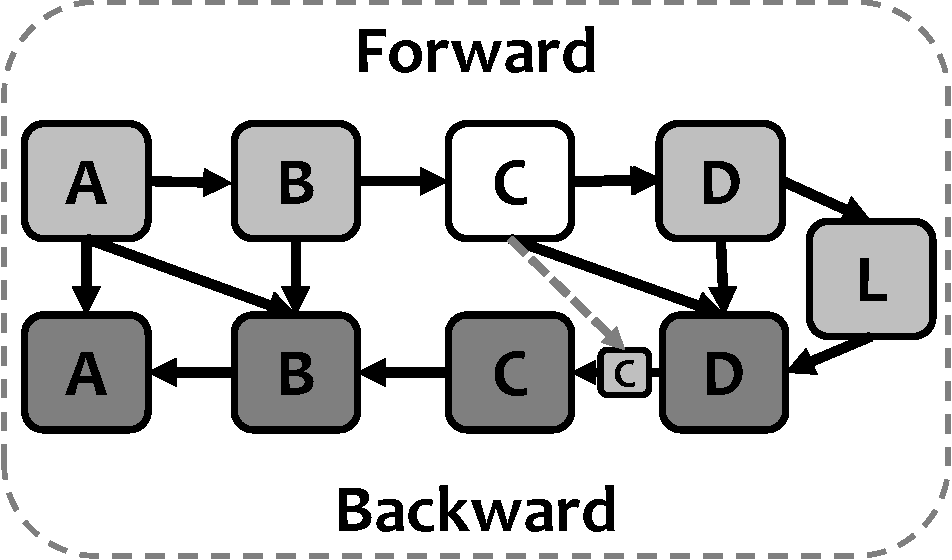
\includegraphics[width=0.45\textwidth]{img/linearize_graph.pdf}
  \caption{Linearized Computational Graph}
  \label{fig: arch}
\end{figure}


However, modern Deep Learning models usually don't naively follow the assumption. 
For example, there exist many residual connections in models such as ResNet~\cite{he2016deep} and Transformer~\cite{transformer}. 
To address the problem, previous works manually rewrite all the PyTorch models needed in their experiments to \texttt{torch.nn.Sequential}. 
However, it is laborsome for researchers and engineers to rewrite models to fit in this framework. 
Fortunately, with \texttt{torch.fx}, we are able to retrieve the forward computational graph and get access to node parents and children. 
Therefore, it is possible for us to do some dependency analysis on the graph structure to determine where to partition the graph to achieve this assumption. 
To clarify our basic rule for network linearization, we should define some of the components in this part.

% \begin{dfn}
% We define some of the concepts related to network linearization here
% \begin{itemize}
%     \item \textbf{Node}: node in the computational graph.
%     \item \textbf{Graph}: computational graph of DNNs, and we assume it is a Directed Acyclic Graph (DAG).
%     \item \textbf{Node group}: the actual "node" for our solver, node groups construct a linearized network.
%     \item \textbf{End of a node group}: during the network linearization, we will examine nodes in the graph following the topological order, then append them to the current node group we are working on. The end of a node group means after appending this node into the working node group, we will move on to the next node group, i.e. the current node could be a partition point for the graph to achieve linearized assumption.
%     \item \textbf{Existing dependencies}: a dynamic dependencies pool. During the process of examing a node in the graph, we will first remove dependencies of this node's parents, and add dependencies of this node's children into this pool. The dependency is expressed by the number of the node's children, and removing dependency is expressed by subtracting the corresponding node's dependency by 1.
% \end{itemize}
% \end{dfn}
\begin{definition}
\textit{We define some of the concepts related to network linearization here}
\begin{itemize}
    \item \textbf{Node}: \textit{node in the computational graph, represents an operation.}
    \item \textbf{Graph}:\textit{ computational graph of neural networks, and we assume it is a Directed Acyclic Graph (DAG).}
    \item \textbf{Node group}: \textit{the actual "node" for our solver, the neural network should be linearized with respect to node groups.}
    \item \textbf{End of a node group}: \textit{during the network linearization, we will examine nodes in the graph following the topological order, then append them to the current node group we are working on. The end of a node group means after appending this node into the working node group, we will move on to the next node group, i.e. the current node could be a partition point for the graph to achieve linearized assumption.
    \item \textbf{Existing dependencies}: a dynamic dependencies pool. While examing a node in the graph, we will first remove dependencies of this node's parents, and add dependencies of this node's children into this pool. The dependency is expressed by the number of the node's children, and removing dependency is expressed by subtracting the corresponding node's dependency by 1.}
\end{itemize}
\end{definition}
With the above definitions, our basic rule is simple: the node can remove all the existing dependencies, i.e. after removing its parents' dependencies, the existing dependencies are all 0, then this node is called the end of a node group. By doing so, it is possible to linearize classic residual networks such as ResNet-152~\cite{he2016deep}.

\subsubsection{Common Node}\label{common_node}

With the utilization of the aforementioned techniques, our solver is able to generate a linearized network automatically. However, the recent transformer-based networks pose a challenge in terms of linearization using the aforementioned basic rule. These networks typically involve constants such as attention masks within their training pipeline, which are used extensively by numerous nodes in the computational graph. Therefore, it is not feasible to linearize such models effectively without specifically processing these nodes. In fact, applying the basic rule to transformer-based networks would result in a node group containing all nodes.

A method for handling this issue was introduced by \cite{lai2022merak}, which involves the use of a common node mechanism to eliminate dependencies associated with nodes like attention masks, thereby enabling linearization of the network. However, their approach to identifying common nodes involves a simplistic threshold-based classification of nodes having a greater number of children than the given threshold. In order to design a more effective common node mechanism, it is necessary to clearly define the characteristics of nodes that can be considered common nodes. The definition of a common node is given below.

\begin{definition}
    \textit{We labeled a node as a common node if it is non-differentiable. For example, the attention mask in PyTorch is non-differentiable as the attention mask is \texttt{bool} type, so the gradient of this kind of node will not be created during training; or operations like \texttt{getattr} and \texttt{getitem} in Python are also non-differentiable.}
    \label{def: common-node}
\end{definition}

As we define the common node, we could further define the propagation of this kind of property throughout the network

\begin{lemma}
    Any node in the graph will be labeled as a common node if any of the following conditions hold:

    \begin{itemize}
        \item All of the parent nodes of this node are labeled as a common node
        \item The operation related to the node is non-differentiable, e.g. \texttt{getattr}, \texttt{getitem}, etc.
    \end{itemize}
    \label{lem:cnodeprop}
\end{lemma}

To initiate the common node propagation, we just need to label the original common node in network input, for example, the attention mask in transformer-based DNNs. Then, with the common node propagation, we are able to expand the common node set and remove dependencies of those nodes during network linearization.

\subsubsection{Full Set of Linearization Rules}

Considering the mechanism mentioned in \ref{linearization} and \ref{common_node}, we are about to give the full set of linearization rules. Before that, there are two more things that should be considered in the linearization process

\begin{itemize}
    \item As mentioned in \ref{modeling}, we include overheads related to communication in our modeling, but we don't need to explicitly add those overheads following the original formula, all we need is to stick those communication nodes to their parents, i.e. include communication nodes in the same group as their parents.
   \item The in-place operation is quite prevalent in modern DNNs, such as standard ResNet structure will set ReLU operation after Batch Normalization to in-place to save memory and time. Those operations together with their parents (those who don't need their output for the backward phase) could be combined so that the memory estimation will be clearer.
\end{itemize}

Therefore, here comes the final network linearization algorithm

% \begin{algorithm}
% \caption{network linearization algorithm}
% \begin{algorithmic}[1]
% \State Input: graph $\mathcal{G}$, common node-set $\mathcal{C}$
% \State Output: linearized graph $\bar{\mathcal{G}}$
% \Function{is\_sink}{$deps\_pool, Node$}
%     \If{$deps\_pool$ is empty and all of $Node.children$ are not in-place operation or communication operation}
%         \State \Return True
%     \Else
%         \State \Return False
%     \EndIf
% \EndFunction
% \State $\bar{\mathcal{G}} \gets []$
% \State $Current\_Node \gets []$
% \State $deps\_pool \gets \{\}$
% \For{$Node$ in $\mathcal{G}$}
%     \If{$Node$ is not placeholder (i.e. input and output)}
%         \For{$Parent$ in $Node.parents$}
%             \If{$Parent$ is not placeholder and common node}
%                 \State $deps\_pool[Parent] -= 1$
%             \EndIf
%         \EndFor

%         \State append $Node$ to $Current\_Node$

%         \If{\Call{is\_sink}{$deps\_pool, Node$}}
%             \State append $Current\_Node$ to $\bar{\mathcal{G}}$
%             \State $Current\_Node \gets []$
%         \EndIf

%         \If{$Node$ satisfies \ref{lem:cnodeprop}}
%             \State append $Node$ to $\mathcal{C}$
%         \Else
%             \State $deps\_pool[Node] \gets len(Node.children)$
%         \EndIf
%     \EndIf
% \EndFor
% \State \return $\bar{\mathcal{G}}$
% \end{algorithmic}
% \end{algorithm}
\begin{algorithm}
\caption{network linearization algorithm}
\KwData{graph $\mathcal{G}$, common node-set $\mathcal{C}$}
\KwResult{linearized graph $\bar{\mathcal{G}}$}
\newcommand{\forcond}{$i=0$ \KwTo $n$}
\SetKwFunction{sink}{is\_sink}
\SetKwProg{Fn}{Function}{:}{}
% \Fn(\tcc*[h]{algorithm as a recursive function}){\FRecurs{some args}}{
\Fn{\sink{$deps\_pool, Node$}}{
\eIf{$deps\_pool$ is empty and all of $Node.children$ are not in-place operation or communication operation}{
\Return True\;
}{\Return False\;
}
}
$\bar{\mathcal{G}} \gets []$\;
$Current\_Node \gets []$\;
$deps\_pool \gets \{\}$\;
\For{$Node$ in $\mathcal{G}$}{
\If{$Node$ is not placeholder (i.e. input and output)}{
        \For{$Parent$ in $Node.parents$}{
            \If{$Parent$ is not placeholder and common node}{
                $deps\_pool[Parent] -= 1$\;
            }
        }
        append $Node$ to $Current\_Node$\;

        \If{\sink{$deps\_pool, Node$}}{
            append $Current\_Node$ to $\bar{\mathcal{G}}$\;
            $Current\_Node \gets []$\;
        }    
        \If{$Node$ satisfies \ref{lem:cnodeprop}}{
            append $Node$ to $\mathcal{C}$\;
        }{
            $deps\_pool[Node] \gets len(Node.children)$\;
        }
    }
}
\Return $\bar{\mathcal{G}}$\;
\end{algorithm}

\subsection{Integrate Two Solvers}

Due to the distinct approaches taken by the two solvers, their training processes' memory requirements are affected. Both solvers aim to optimize for the shortest possible execution time while remaining within the memory budget. If both solvers share the same memory budget, the intra-op parallelism solver's solution will compress the memory within the budget, rendering the activation checkpoint solver redundant. However, modeling the two problems together leads to a significant increase in complexity, making it infeasible to solve within an acceptable timeframe.

To address this issue, we utilize intra-op parallelism to solve the memory budget for a range of values $[(1+\alpha)^n]$ (where n is within the range [0, 9] and $\alpha$ denotes the expansion coefficient). In doing so, we solve a series of memory budgets and input the optimal solution under each budget into the activation checkpoint solver. Ultimately, our final execution plan is determined by identifying the execution plan with the shortest total execution time across different intra-op memory budgets.